% !TEX root = ./document.tex

\documentclass[11pt]{article}

\usepackage{mystyle}
\usepackage{myvars}

%-----------------------------

\begin{document}

  \maketitle

  %-----------------------------
  %  TEXT
  %-----------------------------

  \section{Contexto y Conjunto de Datos}

    \paragraph{}
    En este trabajo se va a realizar un estudio acerca de la diferencia de medias sobre el conjunto de datos \texttt{painkillers}, el cual se refiere a un experimento sobre \emph{Analgésicos Infantiles}. Para ello, se utilizará la técnica de \emph{Análisis de la Varianza (ANOVA)}. Una contextualización más detallada del experimento se describe a partir del siguiente enunciado:

    \paragraph{}
    \say{El departamento de pediatría de un hospital desea analizar la eficacia de cuatro analgésicos infantiles ante las cefaleas. Para ello, realiza un experimento en el que se seleccionan aleatoriamente cinco grupos de cuatro pacientes, de manera que en cada grupo se da un cefalea distinto. A continuación se suministra, también de forma aleatoria, cada analgésico a uno de los pacientes de cada grupo, y se observa el tiempo de remisión de la cefalea, en minutos. Se registran los datos siguientes, en cada uno de los cinco grupos (\texttt{tiempo de remisión}, \texttt{analgésico} y \texttt{cefalea}).}

  \section{Cuestiones}

    \paragraph{}
    En esta sección se incluyen una serie de cuestiones que serán resueltas mediante el estudio del conjunto de datos a partir de la técnica \emph{ANOVA}.

    \subsection{Estudia el tipo de diseño adecuado para esta situación, e identifica las variables, factores y parámetros}

      \paragraph{}
      Tras analizar el contexto del experimento, se sabe que la variable respuesta $Y$ que se utilizará para el \emph{análisis de la varianza} es \texttt{tiempo de remisión}, dado que es la que se utiliza para cuantificar la calidad del tratamiento. En cuanto a las variables a partir de las cuales se pretende explicar el \texttt{tiempo de remisión}, estas son el \texttt{analgésico} y el \texttt{cefalea}.

      \paragraph{}
      Sin embargo, estas no han sido seleccionadas de la misma manera, dado que tal y como se indica en el enunciado, se han fijado $4$ muestras de \emph{a priori} $5$ \texttt{tipos de cefalea}, sobre los cuales aplicar los $4$ tipos de \texttt{analgésico}. Por tanto, podemos interpretar dicha situación diciendo que el factor \texttt{tipos de cefalea} representa un \textbf{bloque} (que denotaremos por $B_\beta$ siendo $\beta \in \{1,2,3,4,5\}$ el identificador de cada uno de los niveles del bloque), y asumiento que el factor \texttt{analgésico} representa un \textbf{tratamiento} (que denotaremos por $T_\alpha $ siendo $\alpha \in \{A, B, C, D\}$ el identificador de cada uno de los niveles del tratamiento).

      \begin{align}
      \label{eq:1f1b_model}
        Y_{ij} = \mu + T_\alpha + B_\beta + \epsilon_{\alpha \beta k} &&
        \begin{split}
          \alpha &\in \{1,...,n_\alpha \} \\
          \beta &\in \{1, ..., n_\beta \} \\
          k &\in \{1,...,  n_{\alpha\beta} \}
        \end{split}
      \end{align}

      \paragraph{}
      Por dichas razones, utilizaremos el modelo de \emph{1 factor + 1 bloque}, el cual se muestra en la ecuación \eqref{eq:1f1b_model}. A este modelo se le ha añadido además la componente $\epsilon_ij$, que representa el error aleatorio y sigue una distribución $N(0, \sigma^2)$, asumiendo que $\sigma^2$ es la misma para todas las observaciones.

      \paragraph{}
      El contraste test de igualdad de medias se describe tal y como se indica en la ecuación \eqref{eq:1f1b_model_test}, que tal y como se puede apreciar, se lleva a cabo teniendo en cuenta únicamente las medias del factor tratamiento, ya que el factor bloque es utilizado únicamente para reducir la variabilidad del modelo.

      \begin{align}
      \label{eq:1f1b_model_test}
        \begin{split}
          H_0 &: \forall i,j \ \mu_i = \mu_j  \\
          H_1 &: \exists i,j \ \mu_i \neq \mu_j
        \end{split} &
        i,j\in \{1,...,n_\alpha\}, \ i \neq j
      \end{align}

      \paragraph{}
      En las figuras \ref{fig:boxplot-analgesico} y \ref{fig:boxplot-cefalea} se muestran los diagramas de caja de la variable respuesta \texttt{tiempo de remisión} agrupados por \texttt{analgésico} y \texttt{cefalea} respectivamente. En estos gráficos se puede apreciar la existencia de diferencias entre las distintas agrupaciones. Por tanto, tiene sentido el estudio del \emph{análisis de la varianza} sobre estas para obtener conclusiones más claras de manera analítica.

      \begin{figure}[!h]
        \centering
        \begin{subfigure}{.5\textwidth}
          \centering
          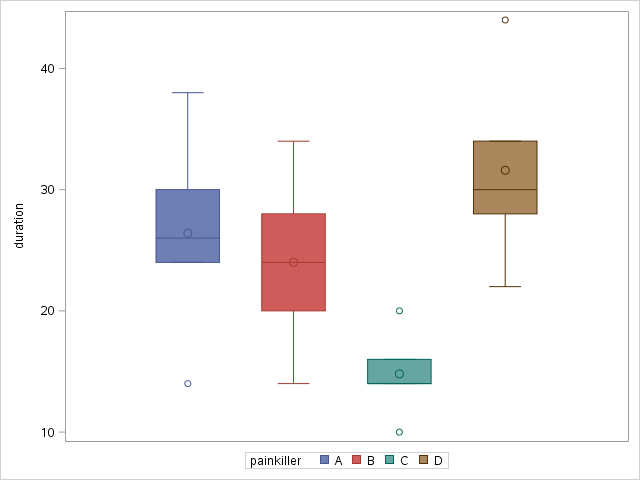
\includegraphics[width=\linewidth]{box-plot-analgesico}
          \caption{\texttt{analgésico}}
          \label{fig:boxplot-analgesico}
        \end{subfigure}%
        \begin{subfigure}{.5\textwidth}
          \centering
          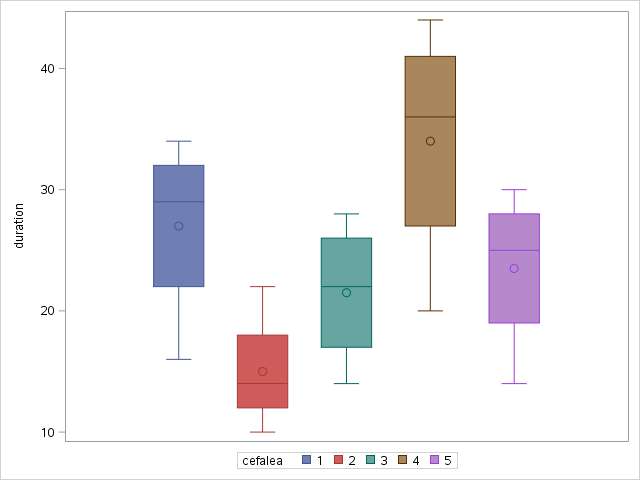
\includegraphics[width=\linewidth]{box-plot-cefalea}
          \caption{\texttt{cefalea}}
          \label{fig:boxplot-cefalea}
        \end{subfigure}
        \caption{Diagramas de cajas}
        \label{fig:boxplot}
      \end{figure}


    \subsection{?`Es adecuado usar las cefaleas como bloques?. ?`Existen diferencias significativas entre los tiempos de remisión de las cefaleas para los distintos analgésicos?}

      \paragraph{}
      A partir del contexto del conjunto de datos se ha asumido que el experimento se ha realizado bloqueando el factor tipo de \texttt{cefalea}. Además, tras visualizar el diagrama de cajas de dicha variable en la figura \ref{fig:boxplot-cefalea} se puede apreciar la existencia de gran variabilidad referida a este factor.

      \begin{figure}[!h]
        \centering
        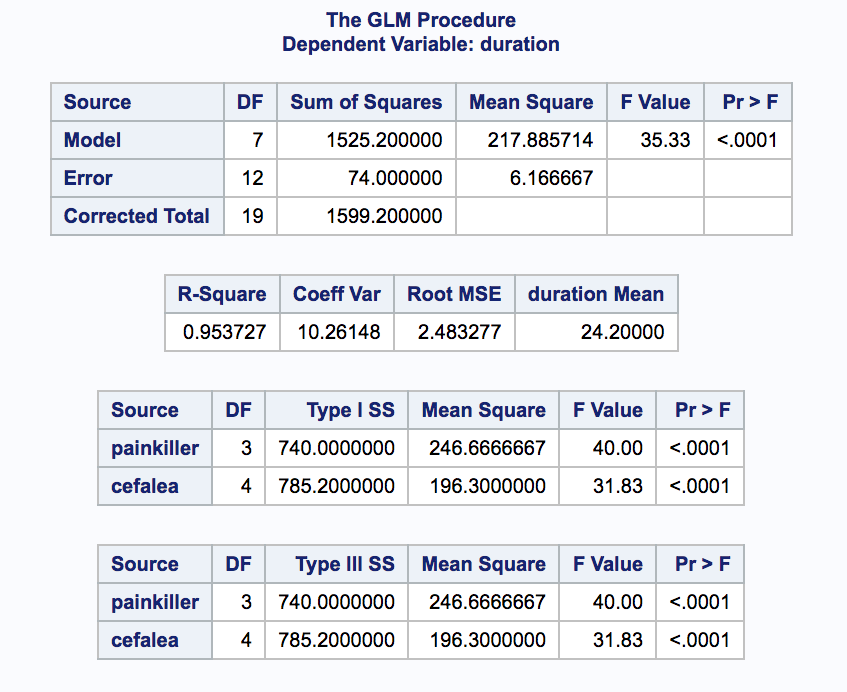
\includegraphics[width=.5\textwidth]{blocks-anova}
        \caption{Resultados del test de igualdad de medias sobre el \emph{ANOVA} de 1 factor y un bloque}
        \label{fig:1f1b-anova-results}
      \end{figure}

      \paragraph{}
      Dicha variabilidad sería tratada como ruido en el modelo, por lo que se ha decidido recoger en un bloque. Los resultados del test de igualdad de medias sobre este modelo se muestran en la figura \ref{fig:1f1b-anova-results}. Tal y como se puede apreciar, la variabilidad recogida por el bloque \texttt{cefalea} es muy elevada, además se rechaza la hipótesis nula por lo que el bloqueo ha sido positivo para el modelo.

      \paragraph{}
      En cuanto a las diferencias entre los distintos tratamientos del factor \texttt{analgésico}, se puede asegurar que estas son significativas con una confianza del $99\%$ debido al rechazo de la hipótesis nula de igualdad de medias.

    \subsection{Estudia gráficamente la existencia de interacción entre analgésico y cefalea}

      \begin{figure}[!h]
        \centering
        \begin{subfigure}{.5\textwidth}
          \centering
          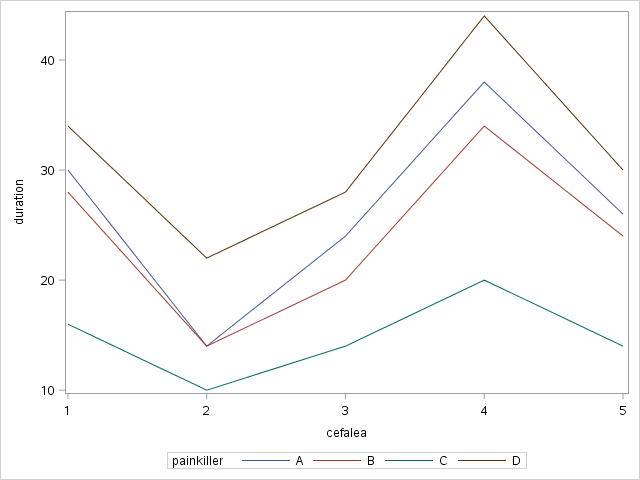
\includegraphics[width=\linewidth]{interaction-analgesico}
          \caption{\texttt{analgésico}}
          \label{fig:interaction-analgesico}
        \end{subfigure}%
        \begin{subfigure}{.5\textwidth}
          \centering
          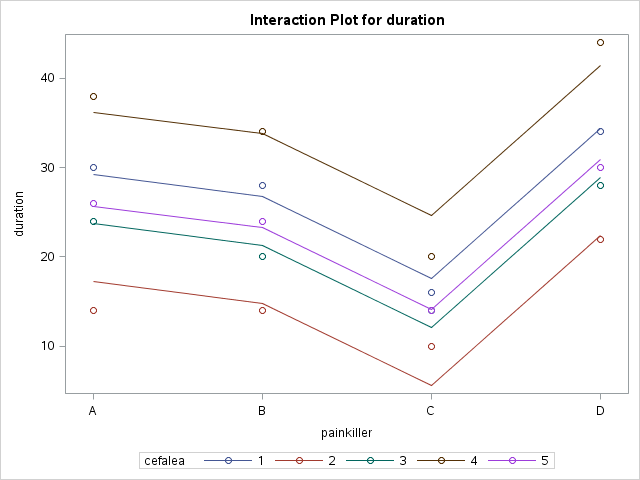
\includegraphics[width=\linewidth]{interaction-cefalea}
          \caption{\texttt{cefalea}}
          \label{fig:interaction-cefalea}
        \end{subfigure}
        \caption{Diagramas de Interacción}
        \label{fig:interaction}
      \end{figure}

      \paragraph{}
      En las figuras \ref{fig:interaction-analgesico} y \ref{fig:interaction-cefalea} se muestran los diagramas de interacción de las variables \texttt{analgésico} y \texttt{cefalea}. A partir de estos, se puede apreciar la no existencia de interacción entre ellos, ya que en ambos casos las rectas permanecen paralelas entre sí. A pesar de ello, estas son traslacciones verticales unas de otras, por lo que se puede asumir la existencia de diferencias entre las distintos tratamientos, pero no la interacción entre ellos.

    \subsection{Determina mediante comparaciones múltiples cuál de los analgésicos es más eficaz}

      \begin{figure}[!h]
        \centering
        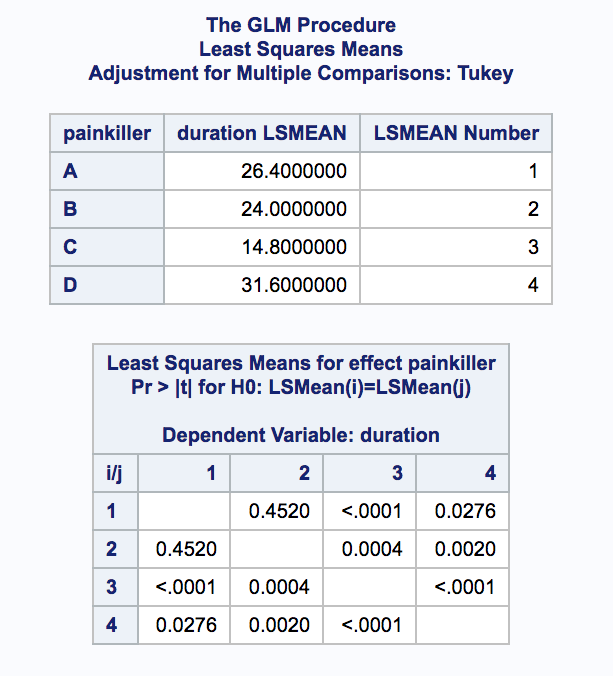
\includegraphics[width=.5\textwidth]{tukey-test}
        \caption{Resultados obtenidos en el método de \emph{Tukey}}
        \label{fig:1f1b-anova-tukey-results}
      \end{figure}

      \paragraph{}
      Como método de comparaciones múltiples se ha escogido \emph{Tukey} por su grado de potencia, con respecto a los requisitos necesarios para su utilización (número igual de observaciones en todos los tratamientos). Los resultados obtenidos se muestran en la figura \ref{fig:1f1b-anova-tukey-results}.

      \paragraph{}
      Tal y como se puede apreciar en los resultados, el \textbf{analgésico C} es el más eficaz para la reducción del tiempo de cefalea, mientras que los analgésicos A y C podrían ser considerados igual de eficaces puesto que no se rechaza la hipótesis de igualdad de medias entre ellos.

    \subsection{Suponiendo que el analgésico A es un placebo, realiza el test de Dunnett}

      \paragraph{}
      El test de \emph{Dunnett} se basa en la comparación de todos los trata respecto de otro denominado \emph{control}. En este caso se ha fijado como control el \emph{analgésico A}, el cual se ha denominado placebo. Los resultados obtenidos en este test se muestran en la figura \ref{fig:1f1b-anova-dunnet-results}.

      \begin{figure}[!h]
        \centering
        \begin{subfigure}{.5\textwidth}
          \centering
          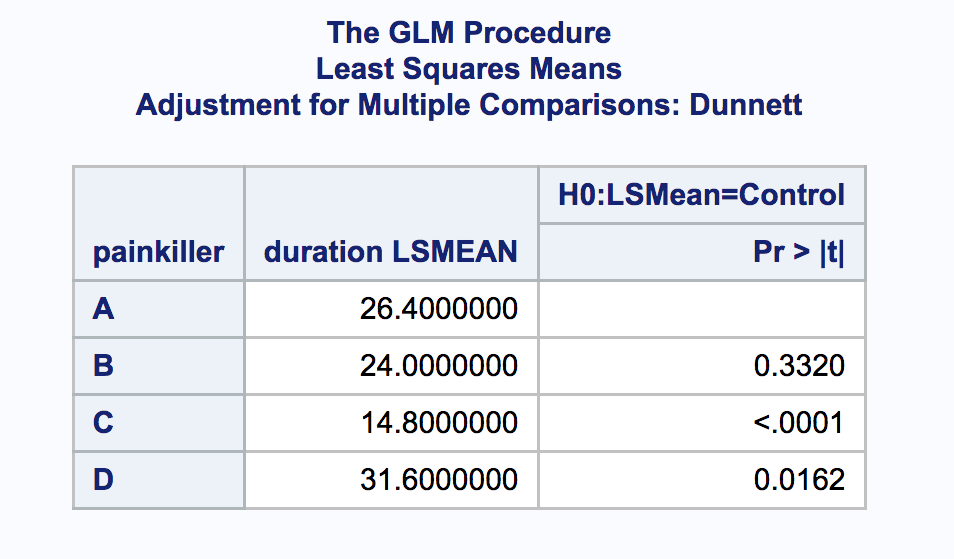
\includegraphics[width=\linewidth]{dunnet-test}
          \caption{Resultados obtenidos en el método de \emph{Dunnett}}
          \label{fig:1f1b-anova-dunnet-results}
        \end{subfigure}%
        \begin{subfigure}{.5\textwidth}
          \centering
          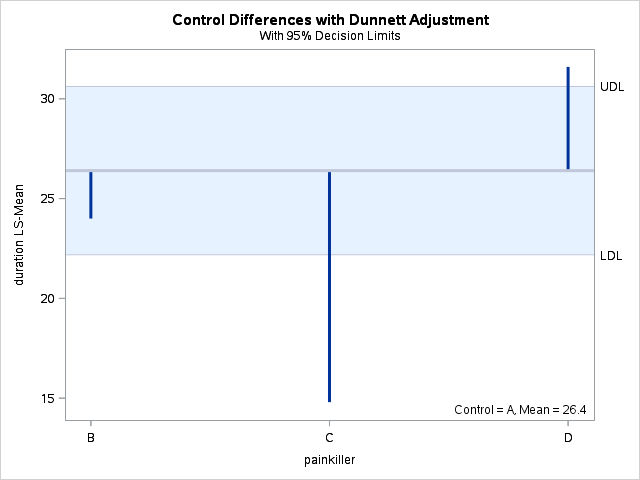
\includegraphics[width=\linewidth]{plot-dunnet}
          \caption{Gráfico de resultados obtenidos en el método de \emph{Dunnett}}
          \label{fig:1f1b-anova-dunnet-plot}
        \end{subfigure}
        \caption{Diagramas de cajas}
        \label{fig:dunnet}
      \end{figure}

      \paragraph{}
      Tal y como se puede apreciar, en este no existen diferencias significativas entre el \emph{placebo} y el \emph{analgésico B}. Sin embargo, si que existen sobre los \emph{analgésicos C y D}

      \paragraph{}
      En la figura \ref{fig:1f1b-anova-dunnet-plot} se muestran los resultados del test de \emph{Dunnett} de manera gráfica, a partir del cual se muestra la \say{dirección} de las diferencias. Por tanto, a partir de este se puede concluir que el \emph{analgésico B} es equivalente al \emph{placebo}, que a partir del \emph{analgésico C} se obtienen tiempos de remisión menores y que con el \emph{analgésico D} los tiempos de remisión aumentan.

    \subsection{Haz un análisis gráfico de los residuos}

      \begin{figure}[!h]
        \centering
        \begin{subfigure}{.5\textwidth}
          \centering
          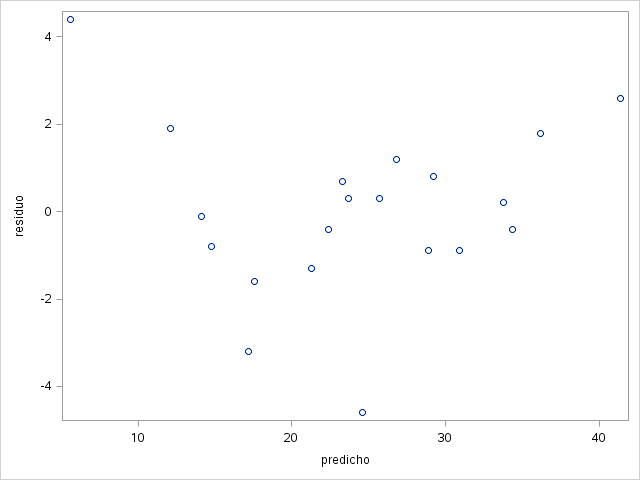
\includegraphics[width=\linewidth]{residuos}
          \caption{Resodios Estándar}
          \label{fig:residuos-standard}
        \end{subfigure}%
        \begin{subfigure}{.5\textwidth}
          \centering
          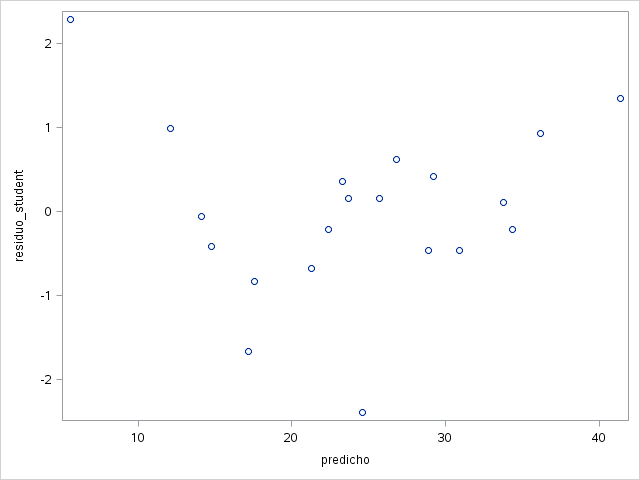
\includegraphics[width=\linewidth]{residuos-student}
          \caption{Residuos Studentizados}
          \label{fig:residuos-student}
        \end{subfigure}
        \caption{Diagramas de Residuos}
        \label{fig:residuos}
      \end{figure}

      \paragraph{}
      En las figuras \ref{fig:residuos-standard} y \ref{fig:residuos-student} se muestran los gráficos de \emph{residuos} y \emph{residuos Studentizados}. A partir de estos, se puede apreciar un sutíl falta de uniformidad en los errores. Sin embargo, esta no debería ser preocupante, debido a la reducida tasa de variabilidad explicada por los mismos. Según el coeficiente de determinación estos explican únicamente el $5\%$ de la variabilidad.

    \subsection{Si los analgésicos se hubieran elegido al azar entre todos los existentes, plantea el modelo adecuado y estima las componentes de la varianza.}

      \paragraph{}
      En este caso se pide tratar el factor \texttt{analgésico} como un factor aleatorio. Por tanto, el modelo a utilizar se define de manera diferente. Este se muestra en la ecuación \eqref{eq:1f_random_model}. A pesar de ser equivalente al anterior a nivel de notación, tiene una interpretación diferente tal y como se verá a continuación.

      \begin{align}
      \label{eq:1f_random_model}
        Y_{ij} = \mu + \Tau_\alpha + B_\beta + \epsilon_{\alpha \beta k} &&
        \begin{split}
          \alpha &\in \{1,...,n_\alpha \} \\
          \beta &\in \{1, ..., n_\beta \} \\
          k &\in \{1,...,  n_{\alpha\beta} \}
        \end{split}
      \end{align}

      \paragraph{}
      En este caso el factor tratamiento $T_\alpha$ pasa a denotarse como $\Tau_\alpha$ y en lugar de representar la diferencia respecto del fator $\alpha$ como un valor escalar, ahora se refiere a una variable aleatoria $\Tau \sim N(0, \sigma_\Tau^2)$. Gracias a esta diferencia, el test \emph{ANOVA} se formula de una manera diferente, en este caso se estudia el efecto de la varianza $\sigma_\Tau^2$, tal y como se indica en la ecuación \eqref{eq:1f_random_model_test}.

      \begin{align}
      \label{eq:1f_random_model_test}
        \begin{split}
          H_0: \sigma^2_\Tau = 0 \\
          H_1: \sigma^2_\Tau > 0
        \end{split}
      \end{align}

      \paragraph{}
      Desde esta perspectiva, ya no tiene sentido estudiar si un tratamiento genera mejores resultados que otro, sino que únicamente se analiza desde el punto de vista de la homogeneidad de la población.

      \paragraph{}
      Tras realizar el \emph{ANOVA} utilizando este modelo, los resultados obtenidos se muestran en las figuras \ref{fig:random-anova-results-1} y \ref{fig:random-anova-results-2}. A partir de dichos resultados se obtiene la conclusión de que se trata de una población heterogénea, es decir, con distintas subpoblaciónes, dado que la hipótesis nula es rechazada con un $p-valor$ muy próximo a cero.

      \begin{figure}[!h]
        \centering
        \begin{subfigure}{.3\textwidth}
          \centering
          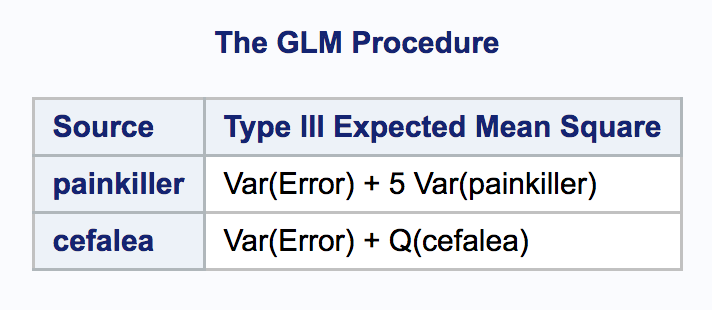
\includegraphics[width=\linewidth]{random-var}
          \caption{Resultados de descomposición de la varianza}
          \label{fig:random-anova-results-1}
        \end{subfigure}%
        \begin{subfigure}{.5\textwidth}
          \centering
          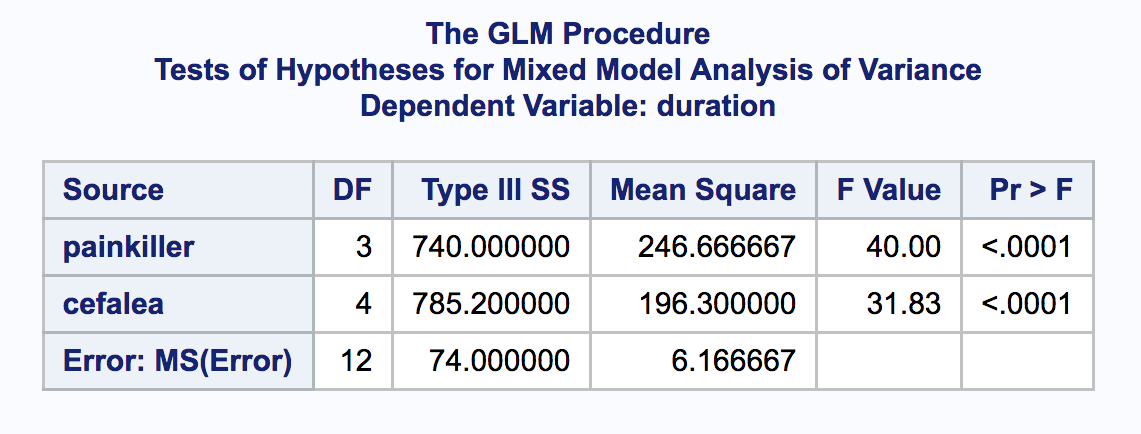
\includegraphics[width=\linewidth]{random-anova}
          \caption{Resultados del test de igualdad de medias}
          \label{fig:random-anova-results-2}
        \end{subfigure}
        \caption{\emph{ANOVA} aleatorizado}
        \label{fig:random-anova}
      \end{figure}

      \paragraph{}
      A partir de estos resultados puede obtenerse una estimación acerca de la varianza del factor \texttt{analgésico}, la cual se realiza a continuación

      \begin{align*}
        Var(\text{Error}) + 5 Var(\text{analgésico}) &= 246.\widehat{6} \\
        Var(\text{Error}) &= 6.1\widehat{6} \\
        &\implies Var(\text{analgésico}) = \frac{246.\widehat{6} - 6.1\widehat{6}}{5} \approx 48.1
      \end{align*}

    \subsection{Plantea el modelo como diseño unifactorial completamente aleatorizado y compara los resultados.}

      \paragraph{}
      En esta sección se realiza el test de igualdad de medias asumiendo la selección complemtamente aleatoria de las observaciones respecto del factor \texttt{analgésico}, de tal manera que se ignora la agrupación por tipos de \texttt{cefalea}. Por tango, el modelo descrito en la ecuación \eqref{eq:1f1b_model} puede reducirse al que se muestra en la ecuación \eqref{eq:1f_model}.

      \paragraph{}
      Sin embargo, en este caso, toda la variabilidad procedente del bloqueo del factor tipo de \texttt{cefalea} se convierte en error no explicado por el modelo. Es decir, ahora lo recoge la variable $\epsilon_{\alpha j}$.

      \begin{align}
      \label{eq:1f_model}
        Y_{ij} = \mu + T_\alpha + \epsilon_{\alpha j}  &&
        \begin{split}
          i &\in \{1,...,n_\alpha\}\\
          j &\in \{1, ..., n_i\}
        \end{split}
      \end{align}

      \paragraph{}
      El test para la igualdad de medias, en este caso se plante de manera equivalente, tal y como se indica en la ecuación \eqref{eq:1f_model_test}. Puesto que la variabilidad procedente del tipo de cefalea ahora es recogido por el error no explicado por el modelo ($\epsilon_{\alpha j}$), las conclusiones que se puedan obtener a partir del estudio del análisis de la varianza deberán ser tomadas con mayor prudencia.

      \begin{align}
      \label{eq:1f_model_test}
        \begin{split}
          H_0 &: \forall i,j \ \mu_i = \mu_j  \\
          H_1 &: \exists i,j \ \mu_i \neq \mu_j
        \end{split} &
        i,j\in \{1,...,n_\alpha\}, \ i \neq j
      \end{align}

      \paragraph{}
      En la figura \ref{fig:simple-anova-results} se muestran los resultados obtenidos tras las realización del estudio \emph{ANOVA} de un factor. Tal y como se puede apreciar, en este caso también se debe rechazar la hipótesis de igualdad de medias, puesto que el \emph{p-valor} del test es muy bajo $(0.0167)$. Por tanto, se puede asegurar con un nivel de confianza del $98\%$ que existen diferencias significativas entre los resultados de los distintos analgésicos.

      \begin{figure}[!h]
        \centering
        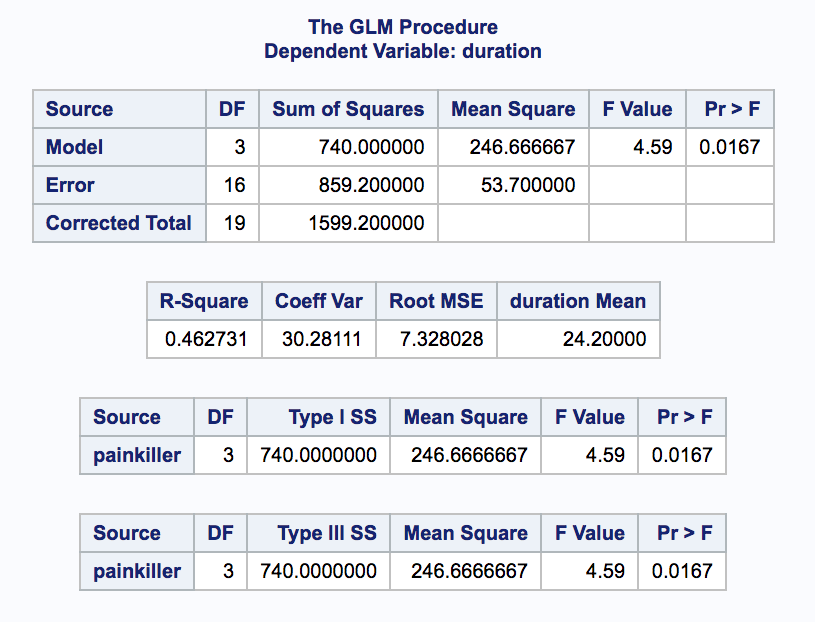
\includegraphics[width=.5\textwidth]{simple-anova}
        \caption{Resultados del teste de igualdad de medias sobre el \emph{ANOVA} de un factor}
        \label{fig:simple-anova-results}
      \end{figure}


      \paragraph{}
      Sin embargo, cabe destacar que estos resultados deben ser tomados con mucha prudencia, debido a que en este caso la variabilidad  del error es mucho mayor que en el modelo de \emph{1 factor + 1 bloque}, variando el coeficiente de determinación $R^2$ del valor $0.95$ a $0.46$. Es decir, con este modelo se explica aproximadamente la mitad de la variabilidad, por tanto no es un modelo acertado para este problema.

  \section{Código Fuente}
  
    \begin{figure}[!h]
      \centering
      \begin{minted}[frame=single,framesep=5pt]{sas}
data painkillers;
  input duration painkiller$ cefalea;
  datalines;
  30 A 1
  28 B 1
  16 C 1
  34 D 1
  14 A 2
  14 B 2
  10 C 2
  22 D 2
  24 A 3
  20 B 3
  14 C 3
  28 D 3
  38 A 4
  34 B 4
  20 C 4
  44 D 4
  26 A 5
  24 B 5
  14 C 5
  30 D 5
;
run;
proc print data=painkillers;
run;
      \end{minted}
      \caption{\emph{Código SAS:} Lectura del conjunto de datos.}
      \label{code:sas_1}
    \end{figure}

    \begin{figure}[!h]
      \centering
      \begin{minted}[frame=single,framesep=5pt]{sas}

proc sgplot data=painkillers;
  vbox duration / group=painkiller;
run;

proc sgplot data=painkillers;
  vbox duration /group=cefalea;
run;
      \end{minted}
      \caption{\emph{Código SAS:} Generación de los diagramas de cajas.}
      \label{code:sas_2}
    \end{figure}

    \begin{figure}[!h]
      \centering
      \begin{minted}[frame=single,framesep=5pt]{sas}
proc glm data=painkillers;
  *class cefalea painkiller;
  class painkiller cefalea;
  model duration=painkiller cefalea ;
  lsmeans painkiller / adjust=tukey;
  lsmeans painkiller / adjust=dunnett;
  random painkiller / test;
  output out=soluc P=predicho R=residuo student=residuo_student;
run;
      \end{minted}
      \caption{\emph{Código SAS:} Realización de ANOVA por bloques.}
      \label{code:sas_3}
    \end{figure}

    \begin{figure}[!h]
      \centering
      \begin{minted}[frame=single,framesep=5pt]{sas}
proc sgplot data=soluc;
  scatter y=residuo x=predicho;
run;

proc sgplot data=soluc;
  scatter y=residuo_student x=predicho;
run;
      \end{minted}
      \caption{\emph{Código SAS:} Generación de diagramas de residuos.}
      \label{code:sas_4}
    \end{figure}
    \begin{figure}[!h]
      \centering
      \begin{minted}[frame=single,framesep=5pt]{sas}
proc glm data=painkillers;
  class painkiller;
  model duration=painkiller;
run;
      \end{minted}
      \caption{\emph{Código SAS:} Realización de ANOVA completamente aleatorizado.}
      \label{code:sas_5}
    \end{figure}
  %-----------------------------
  %  Bibliographic references
  %-----------------------------

  \nocite{rano2017}
  \nocite{sas}

  \bibliographystyle{acm}
  \bibliography{bib}

\end{document}
